\documentclass[conference,a4paper,10pt]{IEEEtran}
\usepackage[T1]{fontenc}
\usepackage[utf8]{inputenc}
\usepackage{newtxtext,newtxmath}
\usepackage{amsmath}
\usepackage{booktabs,array,graphicx}
\usepackage{cite,url,microtype}
\usepackage{tikz}
\usepackage{pgfplots}
\pgfplotsset{compat=1.18}
\ifdefined\pdfinfo
\pdfinfo{/Title (Reassessing Hamming-Weight Leakage in SPHINCS+ FORS) /Author (Eya Frikha)}
\fi
\title{Reassessing Hamming-Weight Leakage in SPHINCS+ FORS}
\author{\IEEEauthorblockN{Eya Frikha}\IEEEauthorblockA{University of Passau, Germany}}
\begin{document}
\maketitle
\begin{abstract}
We revisit the software Hamming-weight leakage analysis of SPHINCS+ FORS reported in a previous Master's thesis. The original correlation implementation tested XOR offsets using logged true secret bytes; its zero-offset result cannot be interpreted as key recovery. We corrected FORS logging to match the implementation's 33 trees and 16-byte selected secrets. In three verified signatures, all 1,584 logged selected-secret bytes, and thus their exact Hamming weights, were available from the public signatures. Separate instrumentation of non-selected FORS leaves produced 99,792 exact byte-level Hamming-weight observations; 811 (0.8127\%) uniquely determined the corresponding byte value. We also evaluated a separate, synthetic PRF hypothesis test: 14 of 16 seed bytes were explicitly assumed known, and all 65,536 possibilities for the remaining two bytes were tested against noiseless Hamming weights at known addresses. The correct suffix was uniquely identified after 12 observations in all 40 trials across fixed and varied test contexts. These findings provide a code-grounded methodological reassessment and a restricted-key validation test, not evidence of practical full-seed recovery or measured physical leakage.
\end{abstract}
\begin{IEEEkeywords}
SPHINCS+, FORS, hash-based signatures, software leakage, Hamming weight, PRF, hypothesis testing, reproducibility.
\end{IEEEkeywords}

\section{Introduction}
SPHINCS+ is a stateless hash-based signature scheme standardized as SLH-DSA; its construction includes FORS, WOTS+, and a hypertree~\cite{nist205,aumasson,bernstein}. Studying its implementation with a software leakage model requires more than observing a correlation: the measured quantity, the hypothesized unknown, and the information already available from a public signature must be distinguished. Otherwise, a reproducible numerical result may be assigned an unsupported security interpretation.

A previous Master's thesis~\cite{frikha2025} evaluated Hamming-weight leakage from the FORS signing path of SPHINCS+-SHA2-128f-simple. It reported zero-valued outputs from a grouped correlation procedure and showed that structural zero positions inflated apparent accuracy. Our re-examination of its C instrumentation and Python analysis identifies three further interpretation problems: the logged layout differs from the configured FORS dimensions; the zero-valued hypothesis is an XOR \emph{offset} tested using the true secret bytes rather than a recovered secret byte; and the selected FORS values being logged already occur in the public signature. The original recovery interpretation therefore requires correction.

This study addresses three questions: (i) can the original selected-secret leakage be reconstructed from public data; (ii) what can exact byte-level Hamming weights determine about non-selected FORS leaf secrets; and (iii) can a deliberately restricted PRF hypothesis test identify an unknown two-byte seed suffix without using that suffix to construct predictions? Our contributions are:
\begin{itemize}
\item \emph{Methodological correction:} a logging layout aligned with 33 FORS trees of 16-byte secrets, verified signing tests, and a precise explanation of the original zero-offset result.
\item \emph{Leakage characterization:} measurements from non-selected leaf derivations and a byte-level analysis of the values consistent with each observed Hamming weight.
\item \emph{Restricted hypothesis validation:} an exhaustive 16-bit PRF suffix test, with 14 seed bytes assumed known, evaluated across fixed and varied synthetic test contexts.
\end{itemize}
All observations are generated in software. We do not claim physical leakage measurement, recovery of an unrestricted signing seed, or a successful Pearson-CPA attack.

\section{Original Model and Methodological Reassessment}
\subsection{Source parameters and corrected logging}
The supplied implementation defines \texttt{SPX\_N=16}, \texttt{SPX\_FORS\_TREES=33}, and FORS height six: each signature selects one 16-byte secret in each of 33 trees, or 528 selected-secret bytes in total. The former logger instead appended two 32-byte buffers per tree, producing 66 records of 32 bytes. Inspection of the included 1,000-signature toy mask shows 16 retained byte positions in each of 33 records and none in the other 33, rather than eight retained positions in every record as stated in the thesis. Its total of 528 retained bytes was correct, but the per-record interpretation was not.

The corrected logger records one 16-byte selected secret, its Hamming-weight values, and one two-byte leaf index per tree. With one keypair and three distinct messages, signing and verification succeeded for all three signatures. The resulting logs contained 1,584 secret bytes, 1,584 leakage bytes, and 198 index bytes, as predicted by the corrected layout.

\subsection{What the original correlation scored}
Let $x_i$ denote a byte read by the analysis from the \emph{ground-truth secret log} in observation $i$. The software logger produces $\ell_i=\operatorname{HW}(x_i)$, where $\operatorname{HW}$ counts set bits. The original thesis wrote $L(g)=\operatorname{HW}(g)$ for a key hypothesis $g$; for fixed $g$, however, this is a constant and cannot form the variable prediction vector needed for Pearson correlation~\cite{brier}. The supplied Python script actually formed the hypothesis-dependent vector
\begin{equation}
 m_i(g)=\operatorname{HW}(x_i\oplus g),\qquad
 r(g)=\operatorname{corr}_i(m_i(g),\ell_i).
 \label{eq:oldscore}
\end{equation}
At $g=0$, $m_i(0)=\ell_i$ for every observation, so $r(0)=1$ whenever the leakage vector has nonzero variance. Thus the selected zero denotes an \emph{XOR offset relative to the known true bytes}, not recovery of a zero-valued secret byte. Moreover, the script initially groups records by leaf index but concatenates those groups for scoring; it does not estimate a separate unknown byte for each index. The former zero-byte recovery rates and decision interpretations therefore cannot be retained as evidence of CPA key recovery.

\subsection{Public-information check}
FORS signing inserts the selected secret value into the signature. In three verified signatures, all $1{,}584/1{,}584$ logged selected-secret bytes matched the corresponding bytes in the public signatures. Computing $\operatorname{HW}$ directly from those public bytes reproduced all $1{,}584/1{,}584$ logged leakage values. For this \emph{exact selected-secret Hamming-weight channel}, the observations therefore reveal no byte-level information beyond those signatures. This conclusion does not address non-selected internal values or physical side channels. The code audit applies to the supplied repository snapshot; its byte-for-byte identity to the original tagged thesis artifact has not been independently established.

\section{Non-Selected Leaf Leakage Characterization}
\subsection{Instrumented derivations}
A temporary copy of the FORS leaf-generation routine was instrumented to record each \emph{non-selected} leaf's global index, 22-byte compressed PRF address, 16-byte derived secret, and exact per-byte Hamming weights. The corrected source remained unchanged; ground-truth bytes were kept private for validation. With 33 trees, $2^6=64$ leaves per tree, and one directly disclosed leaf per tree, the probe recorded $33(64-1)=2{,}079$ non-selected derivations per signature. Three signatures under one keypair verified successfully, yielding 6,237 records and $6{,}237\times16=99{,}792$ measured bytes. All logged weights matched their derived bytes. None of the 6,237 non-selected 16-byte secrets appeared verbatim in the corresponding public signature; this check alone does not prove cryptographic secrecy.

\subsection{Information in the exact-HW channel}
For a derived byte $X\in\{0,\ldots,255\}$, the simulated measurement is $W=\operatorname{HW}(X)$. Given observed weight $w$, the number of compatible byte values is
\begin{equation}
|\{x:\operatorname{HW}(x)=w\}|=\binom{8}{w},\quad x\in\{0,\ldots,255\}.
\label{eq:binomial}
\end{equation}
Weights zero and eight uniquely identify \texttt{0x00} and \texttt{0xFF}; weight four permits 70 values. In the Step 7 data (Fig.~\ref{fig:hist}), 396 observations had weight zero and 415 had weight eight: 811 of 99,792 bytes (0.8127\%) were uniquely specified. All 811 were confirmed using withheld ground truth. This is an exact-channel, \emph{byte-level} result, not seed recovery.

\begin{figure}[t]
\centering
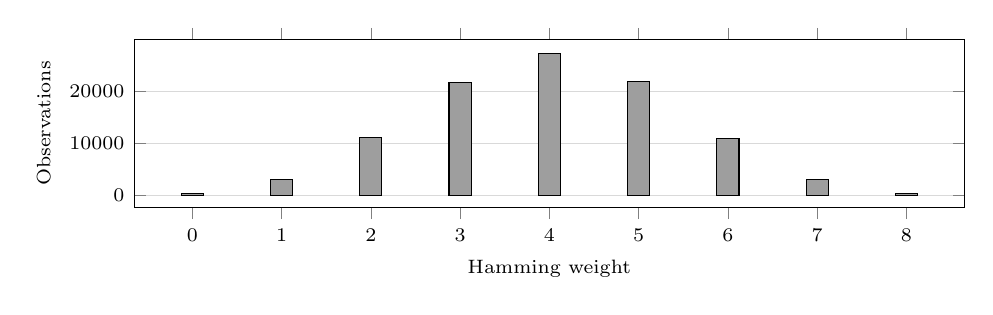
\begin{tikzpicture}
\begin{axis}[width=\columnwidth,height=1.46in,ybar,bar width=8pt,
 xlabel={Hamming weight}, ylabel={Observations},
 xmin=-0.65,xmax=8.65,xtick={0,1,2,3,4,5,6,7,8},
 ymajorgrids=true,grid style={black!15},
 tick label style={font=\scriptsize},label style={font=\scriptsize},
 scaled y ticks=false,ytick={0,10000,20000,30000},
 yticklabel style={/pgf/number format/fixed,/pgf/number format/1000 sep={}}]
\addplot+[fill=black!38,draw=black,mark=none] coordinates {
 (0,396)(1,3099)(2,11050)(3,21664)(4,27201)(5,21885)(6,10958)(7,3124)(8,415)};
\end{axis}
\end{tikzpicture}
\caption{Observed Hamming-weight distribution over the 99,792 non-selected-leaf bytes. Drawn from the uploaded Step 7 aggregate report.}
\label{fig:hist}
\end{figure}

The weight histogram's empirical Shannon entropy was 2.5477 bits. The observed mean $\log_2\binom{8}{W}$ was 5.4523 bits, a count of compatible values on a log scale, \emph{not} an empirical conditional entropy. Under a separate uniformly distributed 8-bit-byte reference, $H(\operatorname{HW}(X))=2.5442$ and $H(X\mid\operatorname{HW}(X))=5.4558$ bits. None measures signing-seed entropy: dependencies among derived bytes and their relation to the seed were not evaluated.

\subsection{Address-based alignment}
In the Step 8 audit, 6,140 cross-signature pairs shared a global leaf index; all 6,140 pairs nevertheless had \emph{different} full PRF addresses. All 6,237 full addresses were distinct. Thus matching an index does not identify repeated processing of the same derived secret. This does not preclude tests across differing \emph{known} addresses, provided predictions model the address-dependent PRF output rather than a fixed unknown byte per index. The next experiment uses addresses explicitly but a \emph{separate synthetic} PRF dataset, not these leaf observations.

\section{Restricted PRF Hypothesis Experiment}
\subsection{Assumptions and hypothesis rule}
This is a \emph{separate synthetic PRF experiment}, not an end-to-end signing attack. The supplied \texttt{prf\_addr()} returns 16 bytes from $\operatorname{SHA256}(s\Vert a)$, where $s$ is a 16-byte seed and $a$ is a 22-byte compressed address. Write $s=p\Vert k^*$, with a 14-byte prefix $p$ \emph{assumed known} and a withheld two-byte suffix $k^*$. This assumption supplies 112 secret-seed bits to the scorer; those bits were not recovered experimentally.

A generator calls the original C PRF with the private test seed at 16 distinct address inputs $a_i$. It reveals only each address and $\ell_i=\operatorname{HW}(P(p\Vert k^*,a_i)[0])$, the exact Hamming weight of the first PRF-output byte. Here $P$ denotes the C PRF. Using only $p$, the addresses, and their noiseless weights, an independent scorer enumerates all 65,536 candidate suffixes. After $t$ observations it retains
\begin{equation}
\mathcal C_t=\{k\in\{0,\ldots,2^{16}-1\}:\;
\operatorname{HW}(P(p\Vert k,a_i)[0])=\ell_i
\;\forall i\le t\}.
\label{eq:surv}
\end{equation}
The scorer does not read $k^*$ or the full PRF outputs. A unique candidate is compared with the private seed \emph{only after scoring}. This is exhaustive exact-match hypothesis filtering, not Pearson CPA or a physical measurement.

\subsection{Experiments and results}
In Step 9, with a fixed known prefix and address set, the surviving candidates fell from 65,536 to 17,841 after one observation, 27 after six, and one after eight; the last matched the private fixture. Step 10 repeated the test 20 times with the same known prefix and addresses but fresh unknown suffixes. Step 11 used 20 new known prefixes, unknown suffixes, and address contexts. Each trial used at most 16 software-generated Hamming weights, with correct uniqueness checked against its private fixture. Table~\ref{tab:success} and Fig.~\ref{fig:success} summarize the checkpoint results.

\begin{table}[t]
\centering
\caption{Correct unique suffix inference (restricted-key tests; 20 trials each).}
\label{tab:success}
\footnotesize
\begin{tabular}{@{}rcc@{}}
\toprule
Obs. & Fixed context & Varied contexts\\
\midrule
1 & 0/20 & 0/20\\
2 & 0/20 & 0/20\\
4 & 0/20 & 0/20\\
6 & 10/20 & 1/20\\
8 & 19/20 & 19/20\\
12 & 20/20 & 20/20\\
16 & 20/20 & 20/20\\
\bottomrule
\end{tabular}
\end{table}

\begin{figure}[t]
\centering
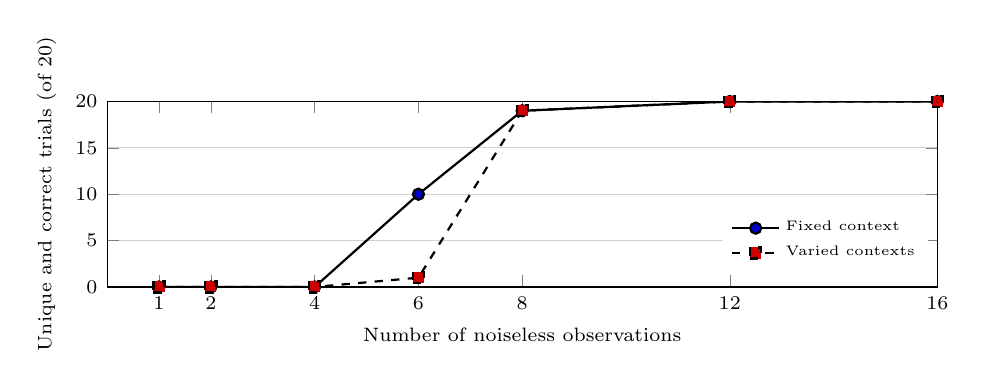
\begin{tikzpicture}
\begin{axis}[width=\columnwidth,height=1.55in,
 xmin=0,xmax=16,ymin=0,ymax=20,
 xtick={1,2,4,6,8,12,16},ytick={0,5,10,15,20},
 xlabel={Number of noiseless observations},
 ylabel={Unique and correct trials (of 20)},
 tick label style={font=\scriptsize},label style={font=\scriptsize},
 ymajorgrids=true,grid style={black!18},
 legend style={font=\tiny,draw=none,at={(0.99,0.25)},anchor=east,fill=white},
 legend cell align=left]
\addplot+[black,mark=*,thick] coordinates {(1,0)(2,0)(4,0)(6,10)(8,19)(12,20)(16,20)};
\addlegendentry{Fixed context}
\addplot+[black,dashed,mark=square*,thick] coordinates {(1,0)(2,0)(4,0)(6,1)(8,19)(12,20)(16,20)};
\addlegendentry{Varied contexts}
\end{axis}
\end{tikzpicture}
\caption{Restricted-key uniqueness by observation count, calculated from Step 10--11 per-trial aggregates. A unique suffix was always checked against the private fixture.}
\label{fig:success}
\end{figure}

After six observations, 10/20 fixed-context and 1/20 varied-context trials had one correct candidate; after eight, 19/20 in each; after twelve, 20/20 in each. In Step 11 the median surviving counts after four, six, and eight observations were 98.5, 4, and 1. The six-observation difference compares distinct, unpaired sets in which multiple factors varied together; it cannot be assigned to any one factor. These results validate the \emph{restricted} noiseless hypothesis test, not recovery of a complete signing seed.

\section{Interpretation, Reproducibility, and Limits}
\emph{Interpretation.} The three experiments address distinct questions. In the selected-secret tests, exact $\operatorname{HW}(X)$ is recomputable from public signature bytes. For non-selected leaves, exact weights restrict possible byte values, including 811 unique determinations; they do not measure seed recovery, because derived bytes depend on a shared seed and addresses. Repeated leaf indices also need not imply repeated PRF inputs. The separate suffix test instead predicts address-dependent values under an explicit 14-byte known-prefix assumption.

\emph{Reproducibility.} Corrected logging and the signing tests use the thesis codebase; the non-selected-leaf probe instruments a temporary copy. The Step 9--11 PRF tests use independent C generator/scorer harnesses and synthetic seed/address fixtures, \emph{not} the signing traces. Exported aggregates were checked: the histogram totals 99,792, the two extreme weights total 811, and both 20-trial series show internally consistent, nonincreasing survivor counts. This verifies the \emph{reports}, not the withheld private fixture values. Exact reproduction of randomized trials requires retained fixtures; fresh trials require the source, patches, and test scripts. The shared evidence archive excludes private secrets.

\emph{Limitations.} Leakage values are exact software outputs, not physical traces. The leaf study includes only three signatures and is not linked to the separate PRF tests as an end-to-end attack. The PRF scorer is given 112 of 128 seed bits and exhausts only the remaining 16. The 20/20 success in each test series describes those restricted trials, not a field success rate. Fixed- and varied-context runs change multiple factors, so the six-observation difference has no isolated causal explanation. Neither Pearson-CPA key recovery, unrestricted seed recovery, nor forgery was demonstrated; original 100,000-signature recovery claims are not used as attack evidence.

\section{Conclusion}
Reassessment of the original SPHINCS+ FORS experiments corrected a logging-layout mismatch and identified the zero-valued correlation result as an XOR offset rather than a recovered byte. In three verified signing tests, selected-secret Hamming weights were fully reconstructable from public signatures. Non-selected-leaf logging yielded 99,792 validated byte weights, with 811 uniquely determining an individual value. Under a separate synthetic model assuming 14 known seed bytes, exhaustive testing of a two-byte PRF suffix identified the correct candidate by twelve noiseless observations in all 40 trials. The work provides a bounded, code-grounded reassessment and reproducible restricted-key validation; no physical or unrestricted key recovery follows.

\begin{thebibliography}{00}
\bibitem{nist205} NIST, \emph{FIPS 205: Stateless Hash-Based Digital Signature Standard (SLH-DSA)}, 2024.
\bibitem{aumasson} J.-P. Aumasson \emph{et al.}, \emph{SPHINCS+: Specification (Submission to NIST PQC, v3.1)}, 2022.
\bibitem{bernstein} D. J. Bernstein \emph{et al.}, ``The SPHINCS+ Signature Framework,'' ACM CCS, full-version preprint, 2019.
\bibitem{frikha2025} E. Frikha, ``Physical Attack Vulnerability of Stateless Hash-Based Signature Schemes: SPHINCS+,'' Master's thesis, University of Passau, 2025.
\bibitem{brier} E. Brier, C. Clavier, and F. Olivier, ``Correlation Power Analysis with a Leakage Model,'' in \emph{CHES}, 2004.
\end{thebibliography}
\end{document}
